To accomplish the goals 

This chapter will illuminate the details of how encryption, authentication, network coding, and ARQ management are implemented in the network
interfaces.

Recall that the architecture of a \gls{noc} consists of a router grid with each node connected to a local processing element through a network
interface (cf. Figure \vref{fig:nocexample}). The 

There are different variants of the protocol, which are explained in detail in Section (insert vref here). While the emphasis lies on network coded
variants, uncoded versions have also been implemented for comparison purposes. However, not all methods have a corresponding uncoded variant.
% TODO: this goes to the overview chapter

Over the course of this chapter, the design of the communication protocol in all variants will be thorougly explained. To begin, fundamental
assumptions about the environment and basic building blocks of the protocol are presented. Since the protocol variants share many elements and differ
mostly in the authentication scheme, the simplest one (uncoded individual authentication) is used to give a step-by-step explanation of the full
protocol. Following this, the other variants are described by drawing upon the differences to uncoded individual authentication.

\section{Design Considerations}
\subsection{Flit Structure}
% Figure of the flit (bar) with header fields (for coded+uncoded)
% Explain purpose of header fields

\subsection{ARQ Structure}

\subsection{Network Coding}\label{sec:designnc}
The coding scheme used in this work slightly differs from the one described above. First, it is applied to unicast transmissions, while traditional
network coding focuses on multicast scenarios \cites{ahlswede00networkflow}{li03linearnc}. Second, only the sender nodes will compute combinations of
different flits, while intermediate nodes merely forward them. The rationale behind this are the tight performance requirements of \glspl{noc}. If
each network node waited for enough flits to perform local encoding before forwarding, routing latencies would increase. Furthermore, the
implementation of local encoding implies additional logic in each router, making their design more complex and entailing a higher chip area
requirement. However, this directly contradicts the \gls{noc} design goals laid out in Section \ref{sec:networkonchipfun} and is thus not considered.
% Only the sender codes
% TODO: mention PNC paper, that we use RLNC, but only senders encode and create generations ("only intra-session network coding")
% TODO: a bit of math and formulas on how NC is done (inspired by previous TUD papers)
% 2 sub-variants: G2C3, G2C4
% Why G2C3 and G2C4? → refer to previous TUD papers

\section{The Protocol}\label{sec:theprotocol}
As mentioned in Section \ref{sec:protocolvariants}, three different communication schemes were envisioned, with the first two subdivided into uncoded
and network coded versions. The remainder of this section provides a comprehensive specification of all variants.

\subsection{Individual Authentication}
\begin{figure}
    \centering
    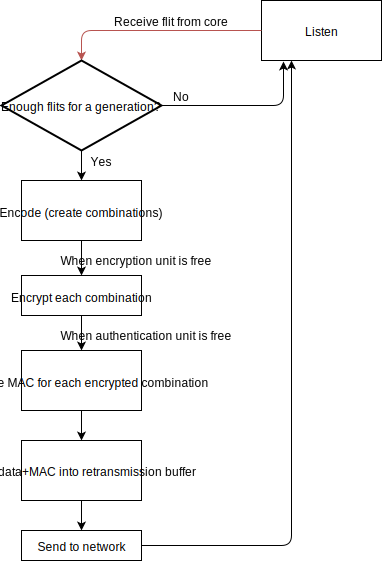
\includegraphics[width=\textwidth]{protocol-flowchart-nc-1}
    \caption[Protocol flow: method 1 coded]{Protocol flow: method 1 coded}
    \label{fig:protchartnc1}
\end{figure}
% uncoded (full explanation), network coded

\subsection{Interwoven Authentication}

\subsection{Full-Generation Authentication}

\section{Routing Strategies}
Mention the perceived/envisioned advantages of adaptive routing (different paths for each flit within the same sender-receiver pair → thanks
to NC enough flits will arrive hopefully even if one path contains a corrupted router).

\subsection{Deterministic XY}
The term \enquote{XY routing} stems directly from the behavior of the routers: flits are only routed along the X axis until they arrive in the column
that the receiver lies in, at which they are routed along the Y axis until reaching the receiver node.
% TODO: figure with a 2D mesh, X and Y arrows on the sides, example path marked for a transmission
\subsection{Dynamic Smart Random}
\subsection{Randomized Oblivious Multi-phase Minimal}
% Both with XY phases and DSR phases
This strategy essentially splits the routing problem into two phases: find a path from sender to proxy node and from proxy to receiver. For each
phase, one of the aforementioned strategies can be applied as is.

\begin{itemize}
    \item Routing Strategies
        \begin{itemize}
            \item Mention routing is general, we are special case of 2D mesh with uniform edge weights → much simpler than arbitrary networks
            \item XY/YX
                \begin{itemize}
                    \item Deterministic path
                    \item Attacker controlling a single router can reliably disrupt communication between certain nodes
                    \item does not distribute flits of a generation across different paths
                \end{itemize}
            \item XY/YX + Valiant
                \begin{itemize}
                    \item Deterministic path only if fixed valiant
                \end{itemize}
            \item Random XorY
            \item Random XorY + Valiant
            \item When writing about this: MANHATTAN DISTANCE (same for XY, YX, random XY, ROMM)
        \end{itemize}
\end{itemize}

\iffalse
\section{Notes}
\begin{itemize}
    \item Encryption/authentication ordering
        \begin{itemize}
            \item Encrypt-then-MAC: best practice. Sequential encrypt/authenticate on sender side, but parallel decrypt/verify
                on receiver side. Advantage: MAC can be computed on receiver side immediately when ciphertext arrives, even when
                MAC flit has not arrived yet (if ARQ is necessary, it can be issued right away)
            \item MAC-then-encrypt: bad. Sequential authenticate/encrypt on sender side and sequential decrypt/verify on receiver
                side.
            \item Encrypt-and-MAC: okay. Parallel encrypt/authenticate on sender side, but sequential decrypt/verify on receiver
                side (overall same latency as Encrypt-then-MAC, but without advantage of fast ARQs)
        \end{itemize}
    \item Uncoded transmission
        \begin{itemize}
            \item no network coding
            \item 2 methods: 1 data flit + 1 MAC flit OR 2 data/MAC split flits
        \end{itemize}
    \item Flit structure
        \begin{itemize}
            \item burst bit, source/target address, mode, address, GID/FID, GEV, payload
            \item mode: define if data/mac/split/arq
        \end{itemize}
    \item Network coded transmission
        \begin{itemize}
            \item Number of flits: G2C3 or G2C4
            \item 3 methods: 1 data flit + 1 MAC flit OR 1 MAC flit per generation OR 2 data/MAC split flits
            \item mention that coded clits are slightly larger due to GEV being embedded → requires wider lanes
        \end{itemize}
    \item ARQs
        \begin{itemize}
            \item Limited number of ARQs per transmission unit (UC: data/MAC pair or split pair, NC: generation)
            \item Timeout of x (e.g. 8) cycles until first ARQ is sent
            \item If limit >1: start larger timeout (→ round-trip of ARQ)
            \item Many different cases, insert some flow diagrams here
            \item The higher the ARQ timeout/limit, the less likely the flit is still in retransmission buffer
            \item → ARQ timeout/limit and retransmission buffer size have to correlate
            \item In the case that we only have 1 ARQ left that we are allowed to send: Wait for any ongoing MAC verifications
                so in case they fail, the flits can be included in the ARQ
        \end{itemize}
\end{itemize}
\fi
